
\chapter{Introduction to Numerical Methods relevant to Thermodynamics}\label{Appendix_NumMethods}


%%%% ETOC
\localtableofcontents

{\it This is not examinable} -- it is here so that you can see where some of the notations, operations and results of earlier sections came from. Details of the contents of this Appendix can be found in \cite{Atkinson_Book_Newton,Atkinson_Book_Interpolation,NumericalRecipes_Interpolation,NumericalRecipes_Newton} or in any text-book of {\it Mathematical or Numerical Methods} for engineering.

%%%
%%% SECTION
%%%
\section{Linear Interpolation}\label{LinearInterpolation}\index{Linear interpolation}

Given a continuous and unknown function $f(x)$, defined at a set of points  $x_{1} < \cdots < x_{i} < \cdots < x_{N}$. Interpolation is the process of determining a polynomial expression to calculate the pair $\left[x_{k}, f\left(x_{k}\right)\right]$ based on neighbours discrete coordinates $\left\{\left[x_{1},f\left(x_{1}\right)\right], \cdots, \left[x_{N},f\left(x_{N}\right)\right]\right\}$. 

Consider a set of discrete data points,
  \begin{center}
    \begin{tabular}{c | c }
        $\mathbf{x}$   & $\mathbf{f\left(x_{i}\right)}$ \\
        \hline
           $x_{1}$ &  $f\left(x_{1}\right)$ \\
           $x_{2}$ &  $f\left(x_{2}\right)$ \\
           $x_{3}$ &  $f\left(x_{3}\right)$ \\
           $x_{4}$ &  $f\left(x_{4}\right)$ \\
    \end{tabular}
  \end{center}
that are a subset of a continuous and smooth function $y=f(x)$ (Fig.~\ref{Appendix:Fig:Interpolation}). Polynomials of order $n\ge 1$ can be generated to represent this function. High-order polynomials can more accurately fit the discrete coordinatess than low-order polynomials. In Fig.~\ref{Appendix:Fig:Interpolation}, let's assume the discrete pairs 
  \begin{displaymath}
     \left\{\left[x_{1},f\left(x_{1}\right)\right], \left[x_{2},f\left(x_{2}\right)\right],\left[x_{3},f\left(x_{3}\right)\right], \left[x_{4},f\left(x_{4}\right)\right]\right\}
  \end{displaymath}
are known, and one wants to determine the value of the function $f$ at $x_{2} < x_{k} < x_{3}$. If the interval $\Delta x= x_{3}-x_{2}$ is sufficiently small, a linear function can be used to fit these coordinates,
   \begin{displaymath}
       f\left(x_{k}\right) = f\left(x_{2}\right) + m\left(x_{k}-x_{2}\right),%\label{LinearInterpolation:Eqn1}
   \end{displaymath}
where 
   \begin{displaymath}
      m = \frc{f\left(x_{3}\right)-f\left(x_{2}\right)}{x_{3}-x_{2}}.
   \end{displaymath}
If $m$ is replaced in the previous equation, %Eqn.~\ref{LinearInterpolation:Eqn1},
   \begin{displaymath}
       f\left(x_{k}\right) = \frc{f\left(x_{2}\right)\left(x_{3}-x_{k}\right) + f\left(x_{3}\right)\left(x_{k}-x_{2}\right)}{x_{3}-x_{2}}.
   \end{displaymath}
   
   \begin{shaded}
      Or for a general case with $x_{a} < x_{k} < x_{b}$,
        \begin{equation}\label{LinearInterpolation:Eqn1}
            f\left(x_{k}\right) = \frc{f\left(x_{a}\right)\left(x_{b}-x_{k}\right) + f\left(x_{b}\right)\left(x_{k}-x_{a}\right)}{x_{b}-x_{a}}.
        \end{equation}
   \end{shaded}

%%% Figure
     \begin{figure}[h]\label{Appendix:Fig:Interpolation}%
        \begin{center}
          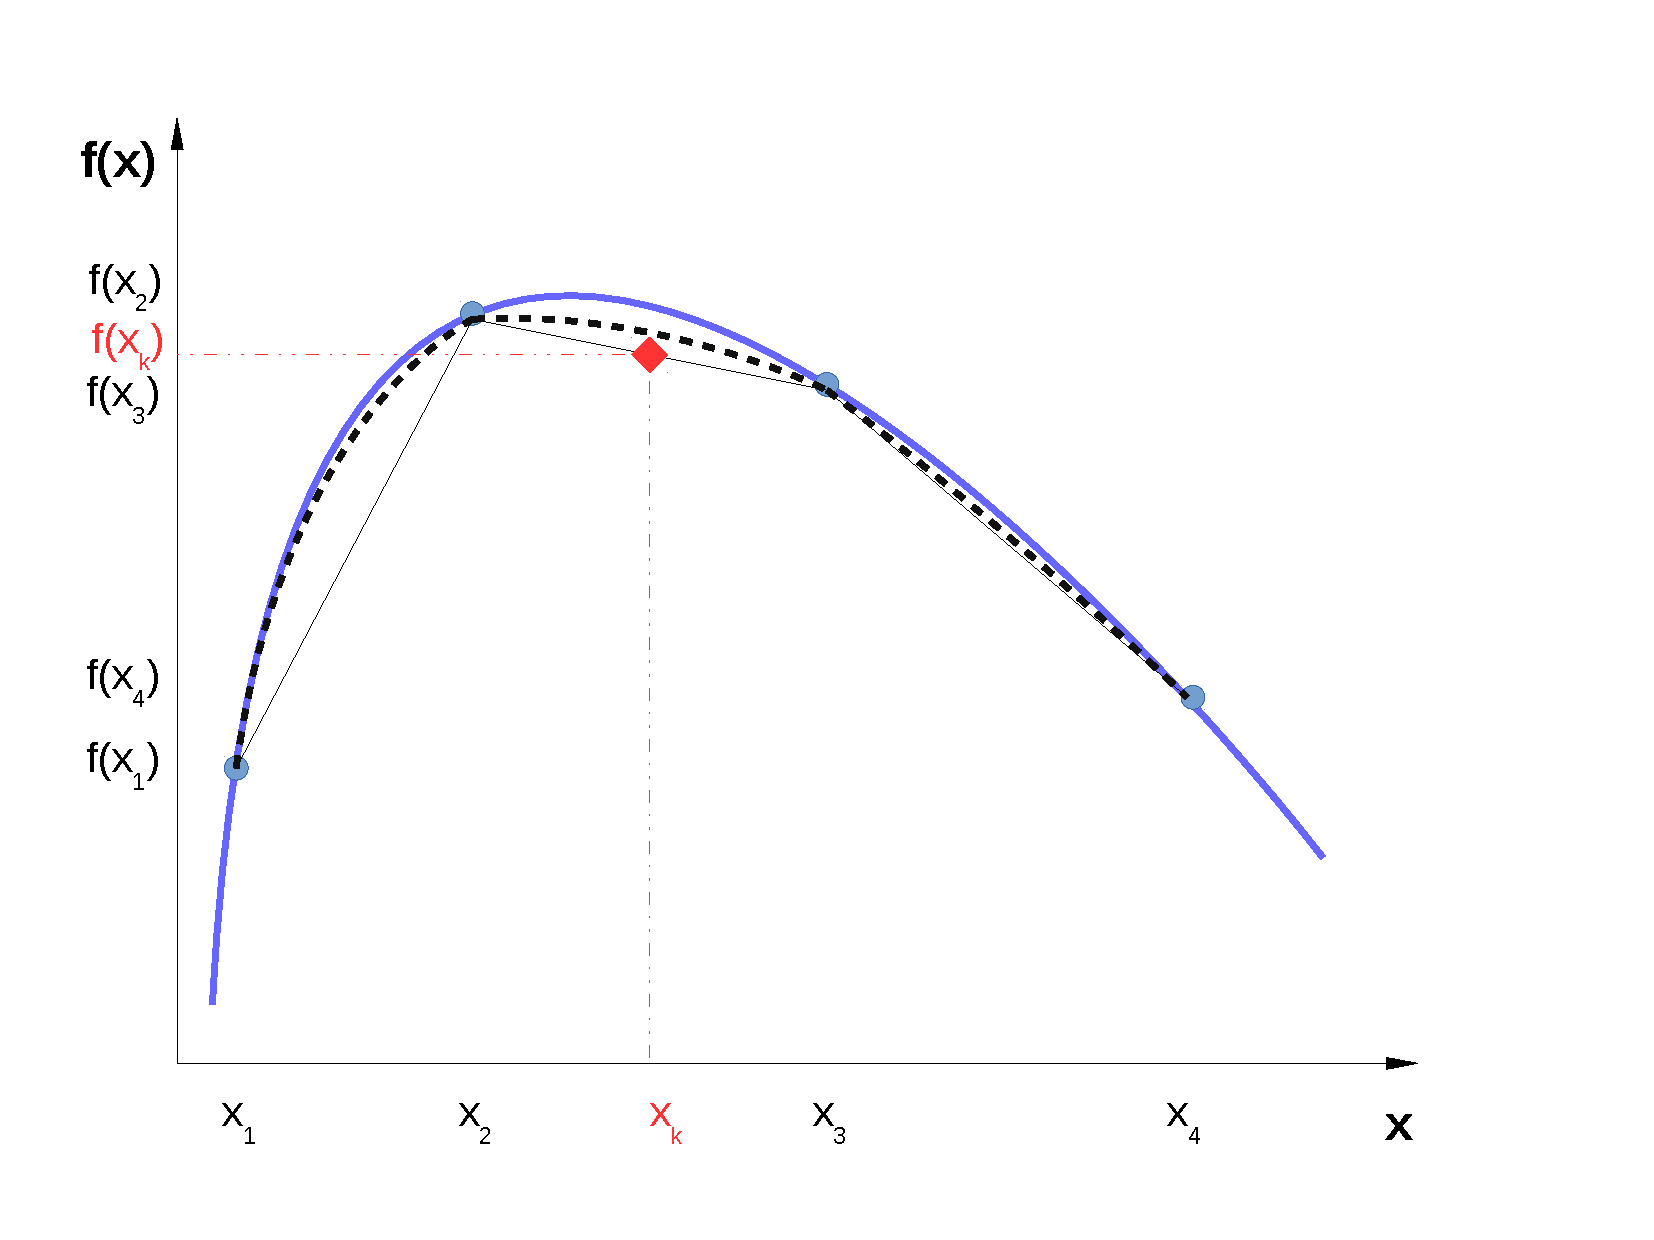
\includegraphics[width=\columnwidth,clip]{./../Pics/Interpolation}
           \caption{Smooth function $f(x)$ (solid blue line) may be more accurately interpolated by a high-order polynomial (black dotted line) than by a low-order polynomial (solid black line).} 
        \end{center}
      \end{figure}

   % Example
   \begin{MyExample}{\begin{center}{\bf Example}\end{center}}
      \begin{example}
         Given a table of values for $f(x)=\tan{x}$ for a few values of $x$,
            \begin{center}
               \begin{tabular}{c | c c c c}
                   $x$        & 1.00   & 1.10   & 1.20   & 1.30   \\
                   \hline
                   $\tan{x}$  & 1.5574 & 1.9648 & 2.5722 & 3.6021 \\
               \end{tabular}
            \end{center}
            Estimate $\tan{(1.15)}$ and $\tan{(1.23)}$.
     \end{example}

% SOLUTION
       \noindent{\bf Solution:} For $\left(x_{a}=1.10\right) < \left(x_{k}=1.15\right) < \left(x_{b}=1.20\right)$,
               \begin{eqnarray}
                  f\left(x_{k}\right) &=& \frc{f\left(x_{a}\right)\left(x_{b}-x_{k}\right) + f\left(x_{b}\right)\left(x_{k}-x_{a}\right)}{x_{b}-x_{a}} \nonumber \\
                                     &=& \frc{1.9648\times(1.20-1.15) + 2.5722\times(1.15-1.10)}{1.20-1.10} = 2.2685 \nonumber
               \end{eqnarray}

For  $\left(x_{a}=1.20\right) < \left(x_{k}=1.23\right) < \left(x_{b}=1.30\right)$,
               \begin{eqnarray}
                  f\left(x_{k}\right) &=& \frc{f\left(x_{a}\right)\left(x_{b}-x_{k}\right) + f\left(x_{b}\right)\left(x_{k}-x_{a}\right)}{x_{b}-x_{a}} \nonumber \\
                                     &=& \frc{2.5722\times(1.30-1.23) + 3.6021\times(1.23-1.20)}{1.30-1.20} = 2.8812 \nonumber
               \end{eqnarray}
   \end{MyExample}

   % Example
   \begin{MyExample}{\begin{center}{\bf Example}\end{center}}
      \begin{example}
         Calculate specific volume $\left(v, \text{in m}^{3}\text{.kg}^{-1}\right)$, internal energy $\left(u, \text{in kJ.kg}^{-1}\right)$ and entropy $\left(s, \text{in kJ.(kg.K)}^{-1}\right)$ of saturated water vapour at 133.45$^{\circ}$C.
     \end{example}

% SOLUTION
       \noindent{\bf Solution:} From Appendix~\ref{Appendix:Saturated_SH_Tables} (Table A-2), for $T_{a}(=130.0) < T_{k} (= 133.45) < T_{b} (=140.0)^{\circ}C$, thus:
               \begin{eqnarray}
                  v\left(T_{k}\right) &=& \frc{v\left(T_{a}\right)\left(T_{b}-T_{k}\right) + v\left(T_{b}\right)\left(T_{k}-T_{a}\right)}{T_{b}-T_{a}} \nonumber \\
                                     &=& \frc{0.6685\times(140.0-133.45) + 0.5089\times(133.45-130.0)}{140.0-130.0} = 0.6134 \text{ m}^{3}\text{.kg}^{-1}\nonumber \\
                                     && \nonumber \\
                  u\left(T_{k}\right) &=& \frc{u\left(T_{a}\right)\left(T_{b}-T_{k}\right) + u\left(T_{b}\right)\left(T_{k}-T_{a}\right)}{T_{b}-T_{a}} \nonumber \\
                                     &=& \frc{2539.9\times(140.0-133.45) + 2550.0\times(133.45-130.0)}{140.0-130.0} = 2543.39 \text{ kJ.kg}^{-1}\nonumber \\
                                     && \nonumber \\
                  s\left(T_{k}\right) &=& \frc{s\left(T_{a}\right)\left(T_{b}-T_{k}\right) + s\left(T_{b}\right)\left(T_{k}-T_{a}\right)}{T_{b}-T_{a}} \nonumber \\
                                     &=& \frc{7.0269\times(140.0-133.45) + 6.9299\times(133.45-130.0)}{140.0-130.0} = 6.9934 \text{ kJ.}\left(\text{kg.K}\right)^{-1}\nonumber 
               \end{eqnarray}
   \end{MyExample}


%%%
%%% SECTION
%%%
\section{Root-Finder Methods}\label{Section:RootFinderMethods}\index{Root-Finder Methods}

%%% SUBSECTION
\subsection{Motivation}
Given a smooth, {\it continuous} and {\it fully differentiable} function 
  \begin{displaymath}
     y = f(x) \hspace{3cm} \text{ with } x\in\mathbb{R}.
  \end{displaymath}
We aim to find the root $x=\psi$ of the function 
  \begin{displaymath}
     f(x) = 0.
  \end{displaymath}
The first step is to estimate $x_{0}$ that results in $f\left(x_{0}\right)\neq 0$ and may lead to a new estimate $x_{1}$. The procedure is repeated until $f\left(x_{n}\right)\rightarrow 0$ (\ie $x_{n}\approx\psi$), where $n$ is the number of repetitions (or {\it iterations}). There are several methods designed to solve non-linear equations, i.e., find the rrot of the function, here we will focus on the most popular {\it Newton-Raphson} method that combines simplicity and power.


%%% SUBSECTION
\subsection{Newton-Raphson Iterative Method}\label{Section:RootFinderMethods:NewtonRaphson}\index{Root-Finder Methods!Newton-Raphson method}
Let's assume that $x_{0}$ is a good estimate of the root$\psi$ and $\psi = x_{0} + h$. Since the root of the function $f(x)$ is $\psi$ and $h = \psi 0 x_{0}$, $h$ represents the distance between the initial estimate (or guess) and the root. Assuming $h$ is very (or {\it infinitesimal}) small, we can linearly approximate the function,
   \begin{displaymath}
        f\left(\psi\right) = 0 = f\left(x_{0}+h\right) \approx f\left(x_{0}\right) + h f'\left(x_{0}\right).
   \end{displaymath}
Therefore, except if $f'\left(x_{0}\right)$ is close to $0$, 
   \begin{displaymath}
        h \approx -\frc{f\left(x_{0}\right)}{f'\left(x_{0}\right)} \hspace{.3cm} \Longrightarrow \hspace{.3cm} \psi = x_{0} + h \approx x_{0} -\frc{f\left(x_{0}\right)}{f'\left(x_{0}\right)}.
   \end{displaymath}
%%% Figure
     \begin{figure}[h]\label{Appendix:Fig:NewtonRaphson}%
        \begin{center}
         \vbox{
           \hbox{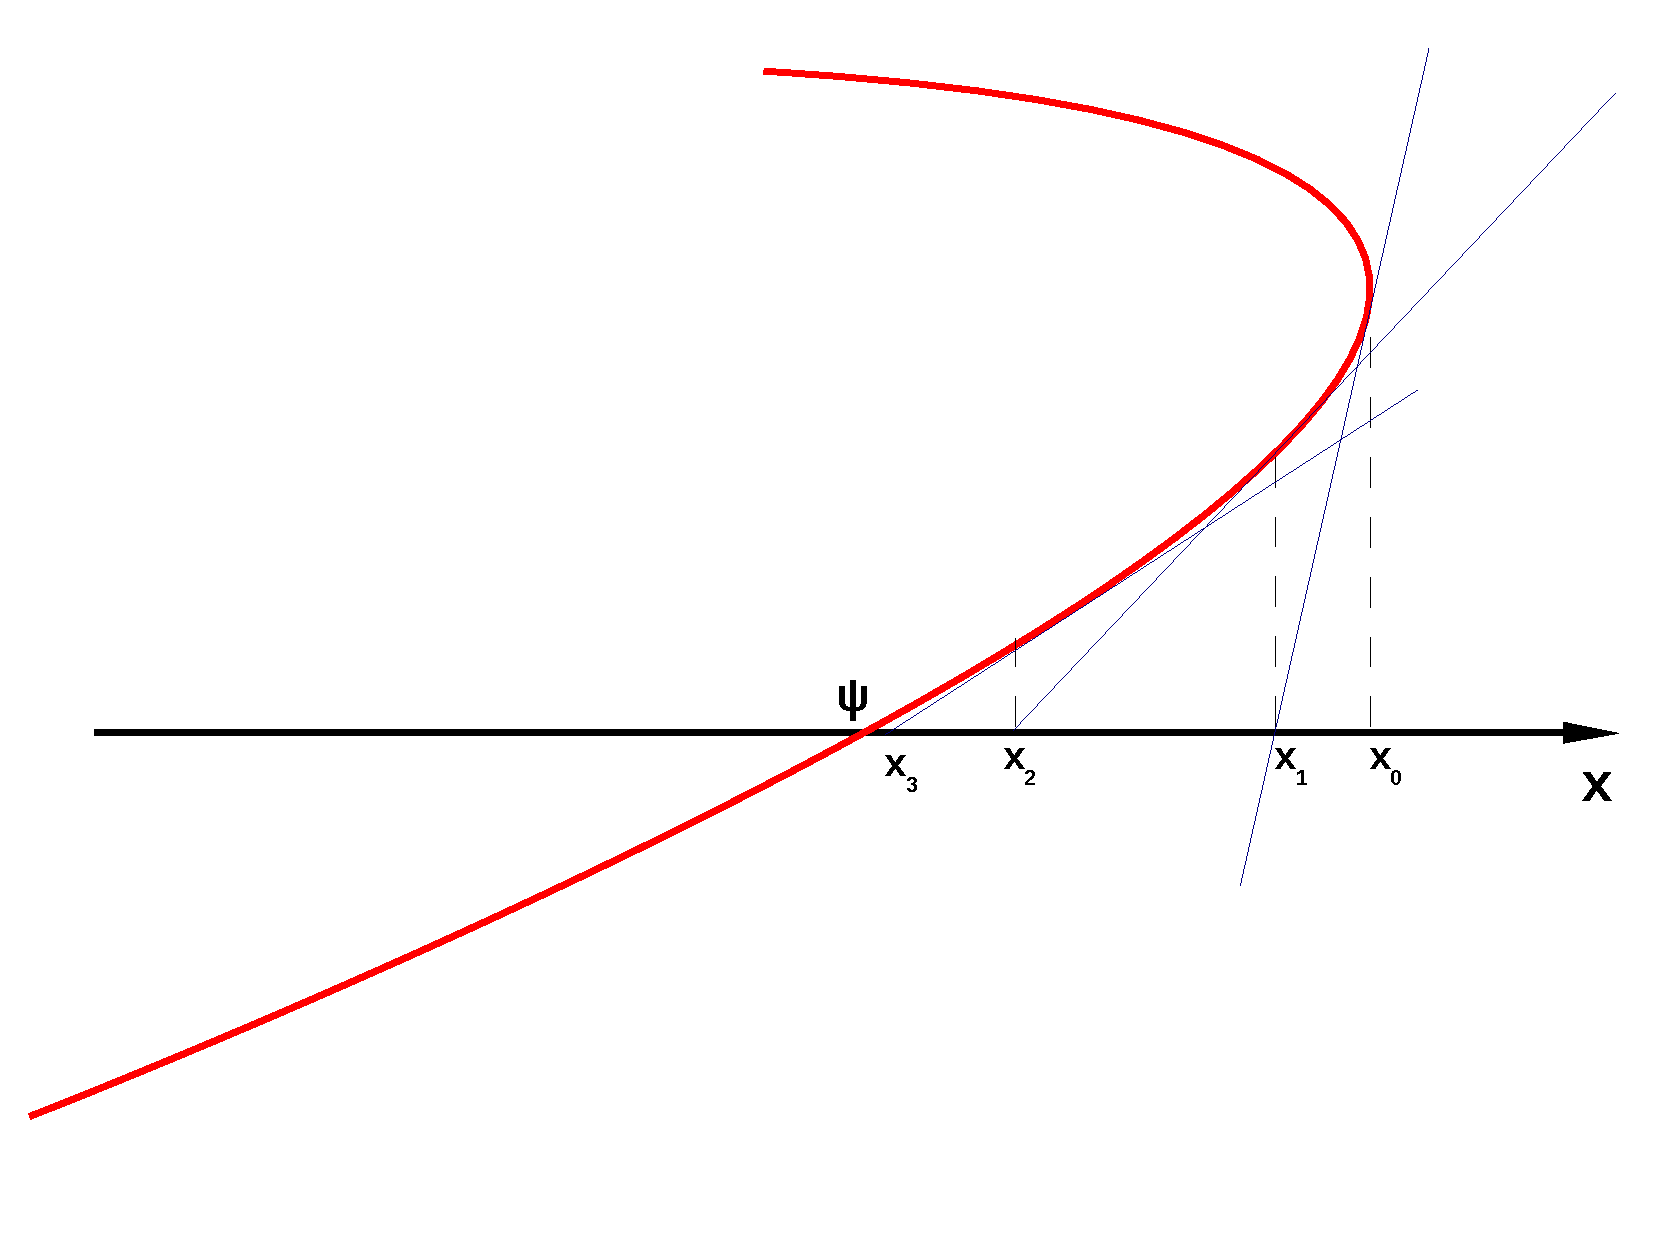
\includegraphics[width=\columnwidth,height=10cm]{./../Pics/NewtonRaphson2}}
           \hbox{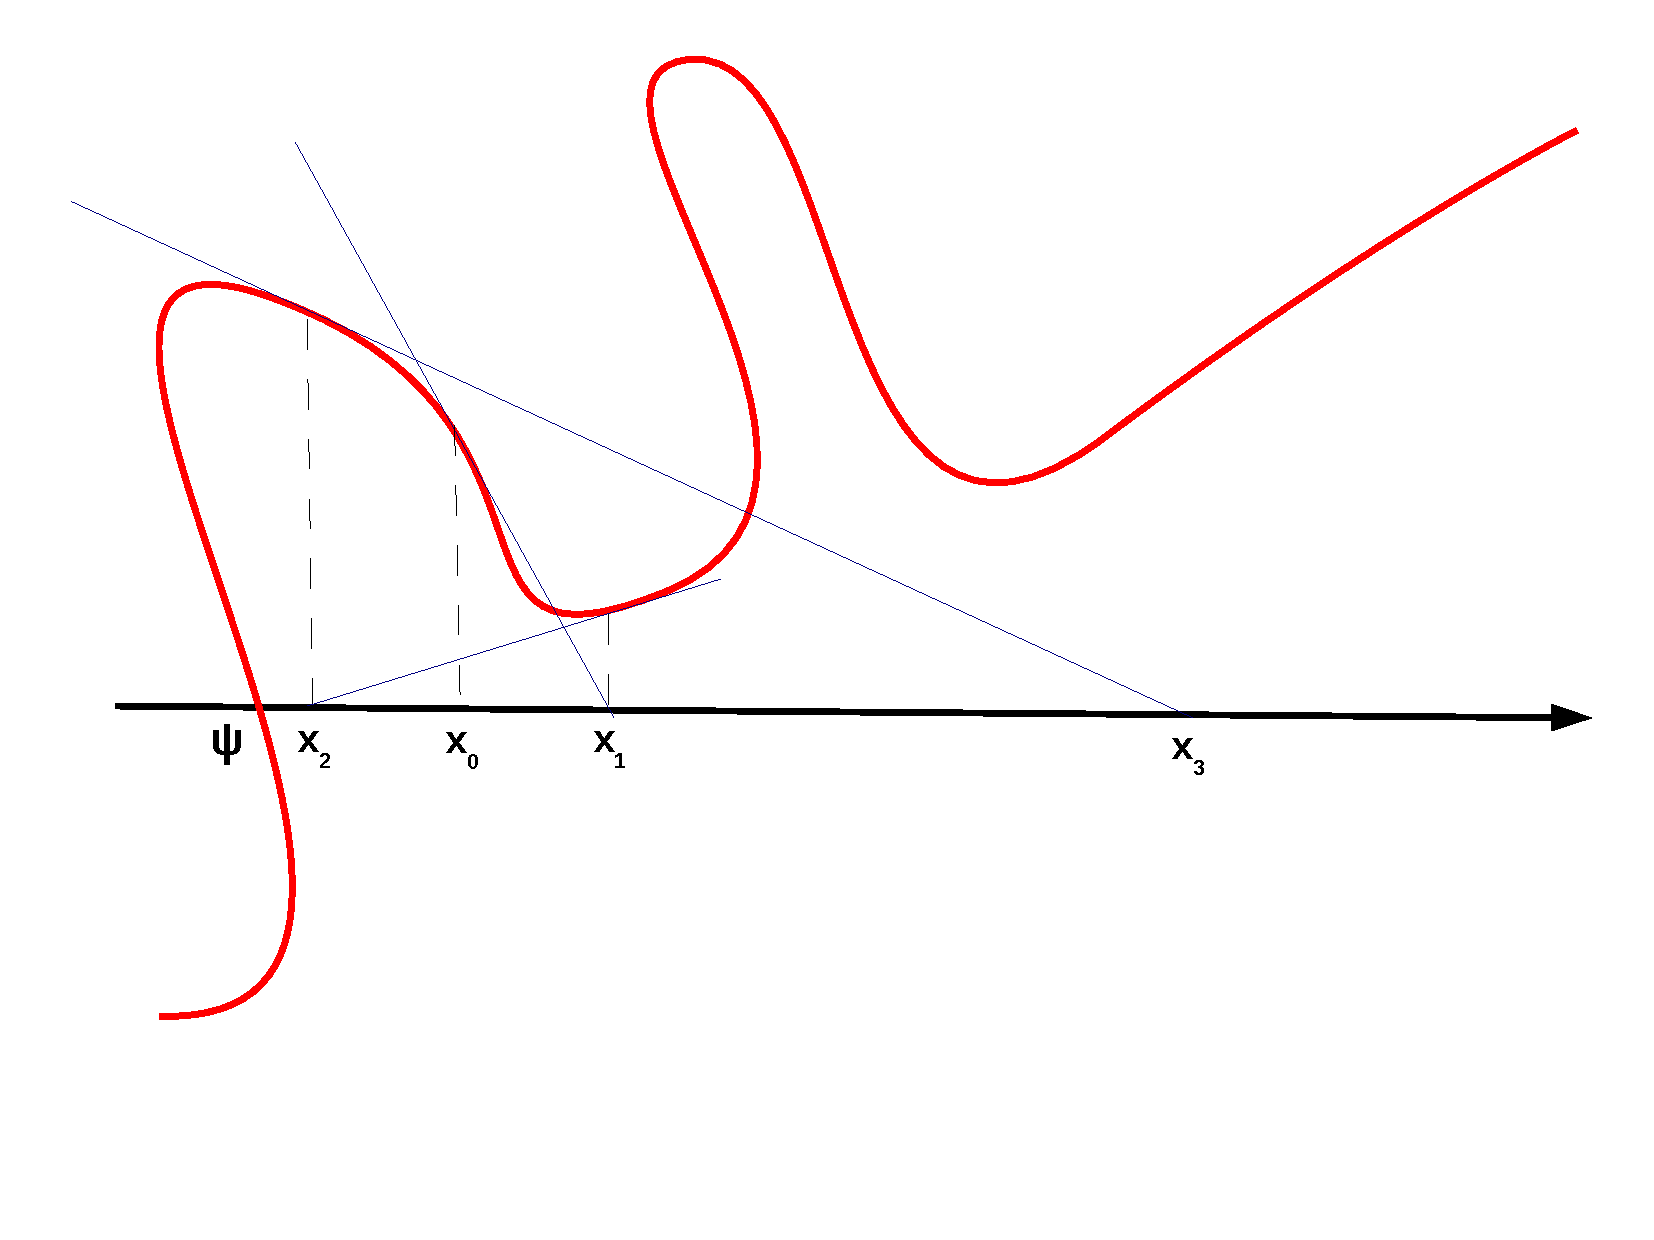
\includegraphics[width=\columnwidth,height=10cm]{./../Pics/NewtonRaphson3}}}
           \vspace{-1cm}
           \caption{Graphic representation of the Newton-Raphson iterative method: (top) solution of the smooth and continuous function $f(x)$ (solid red line) is approximated from the initial estimate $x_{0}$ to the final solution $x=\psi$; (bottom) initial estimate $x_{0}$ is far away from the root $\psi$ and the solution may diverge. Blue solid lines are tangent of the function at $x_{i}$.} 
        \end{center}
      \end{figure}
%
This expression represents an improvement of the original estimate, i.e.,  
   \begin{displaymath}
        x_{1} = x_{0} -\frc{f\left(x_{0}\right)}{f'\left(x_{0}\right)}.
   \end{displaymath}
The next estimate, $x_{2}$, is obtained from $x_{1}$, 
   \begin{displaymath}
        x_{2} = x_{1} -\frc{f\left(x_{1}\right)}{f'\left(x_{1}\right)}.
   \end{displaymath}

   \begin{shaded}
      We can generalise this expression for the $n-${\it th iteration},
         \begin{equation}
            x_{n+1} = x_{n} -\frc{f\left(x_{n}\right)}{f'\left(x_{n}\right)}.\label{NewtonRaphson:Eqn1}
         \end{equation}
   \end{shaded}

Figure~\ref{Appendix:Fig:NewtonRaphson}(a) shows a geometrical representation of the Newton-Raphson iterative method, where $m=f(x)$ is the tangent (blue) line at the coordinate pair $\left[x_{0},f\left(x_{0}\right)\right]$,
   \begin{displaymath}
     m = f\left(x_{0}\right) + \left(x-x_{0}\right)f'\left(x_{0}\right).
   \end{displaymath}
Let $x_{1}$ be the {\it x-intercept} of the tangent line, therefore
   \begin{displaymath}
     x_{1} = x_{0} - \frc{f\left(x_{0}\right)}{f'\left(x_{0}\right)}
   \end{displaymath}
The tangent line is a geometrical representation of the Newton-Raphson iterative method, Eqn.~\ref{NewtonRaphson:Eqn1}, as the estimates gradually tend to the root $\psi$ of the function. As it can be seen in the Fig.~\ref{Appendix:Fig:NewtonRaphson}(b), if the initial estimate $x_{0}$ is not close enough of the root $\psi$, the solution may not {\it converge}. In fact, the Newton-Raphson iterative method works most of the time if the initial estimate is {\it good enough}.

 From the {\it mean value theorem} (Theorem~\ref{Appendix:MeanValueTheorem}), let the function $f(x)$ be such that, 
   \begin{enumerate}[(a)]
      \item it is continuously differentiable in some open interval containing the solution $x=\psi$;
      \item $\left|f'(\psi)\right| < 1$.
   \end{enumerate}
Then there is a number $\epsilon > 0$ such that the iteration $x_{k+1}=f\left(x_{k}\right)$ {\it converges} whenever $x_{0}$ is chosen in $\left|x_{0}-\psi\right|\leq\epsilon$.

For bounded $x\in\mathbb{R}$ (\ie contained in the interval $a\leq x \leq b$), if $f''(x)$ exists and is continuous on $[a,b]$ and $\psi$ is a root of $f(x)$, that is, $f(\psi)=0$ and $f'(\psi)\neq0$. Thus for a function $g(x)$
    \begin{displaymath}
        g(x) = x - \frc{f(x)}{f'(x)}
    \end{displaymath}
with
    \begin{displaymath}
        g'(x) = 1 - \frc{[f'(x)]^{2} - f(x)f''(x)}{[f'(x)]^{2}} = \frc{f(x)f''(x)}{[f'(x)]^{2}},
    \end{displaymath}
and
    \begin{displaymath}
        g'(\psi) = \frc{f(\psi)f''(\psi)}{[f'(\psi)]^{2}}=0, \text{ since } f(\psi) = 0 \text{ and } f'(\psi) \neq 0
    \end{displaymath}
As $g'(x)$ is continuous, this means that there is a small neighbourhood around the root $x=\psi$ such that for all points $x$ in that neighbourhood, $\left|g'(x)\right|<1$.  Therefore, if $g(x)$ is chosen as above and the initial estimate $x_{0}$ is chosen {\it sufficiently close to the root} $x=\psi$, then the Newton-Raphson method is {\it guaranteed to converge}. 

Algorithm~\ref{Algorithm:NewtonRaphson} highlights the steps towards find the root of a function $f(x)$.

\begin{algorithm}[h]%\scriptsize
   \SetKwData{Left}{left}\SetKwData{This}{this}\SetKwData{Up}{up}
   \SetKwFunction{Union}{Union}\SetKwFunction{FindCompress}{FindCompress}
   \SetKwInOut{Input}{Input}\SetKwInOut{Output}{Output}\SetKwInOut{Calculate}{Calculate}\SetKwInOut{Set}{Set}\SetKwInOut{Adjust}{Adjust}\SetKwInOut{Assumption}{Assumption}

      \Input{Given the function $f(x)$, the initial estimate $x_{0}$, the error tolerance $\epsilon$ and the maximum number of iterations $N$:}
      \Output{An approximation to the root $x=\psi$}

      \Assumption{$x=\psi$ is a root of $f(x)$}

      \For{$k \leftarrow 0$ \KwTo $N$}{
             \Calculate{ $f\left(x_{k}\right)$ and $f'\left(x_{k}\right)$ }

             \Calculate{ $x_{k+1} = x_{k} - \frc{f\left(x_{k}\right)}{f'\left(x_{k}\right)}$ }

             \eIf{ $k == N$}{
                             {\it Calculation has \underline{not converged}. Modify the initial estimate $x_{0}$.} 
                   }{
                     \If{ $\left|f\left(x_{k}\right)\right| \leq \epsilon$ {\bf or} $\frc{\left|x_{k+1}-x_{k}\right|}{\left|x_{k}\right|} \leq \epsilon$ }{
                          {\it Stopping criteria} achieved. The root of function $f(x)$ is $\psi = x_{k+1}$
                          } }
          }
 \caption{Newton-Raphson method algorithm.}\label{Algorithm:NewtonRaphson}
\end{algorithm}

%%% SUBSECTION
\subsection{Secant Iterative Method}\label{Section:RootFinderMethods:Secant}\index{Root-Finder Methods!Secant method}
The Secant method is essentially the same as Newton-Raphson, however the derivative $f'(x)$ is approximated by a finite difference based on the current and the previous estimate for the root,
   \begin{displaymath}
       f'\left(x_{n}\right) \approx \frc{f\left(x_{n}\right) - f\left(x_{n-1}\right)}{x_{n}-x_{n-1}}
   \end{displaymath}

   \begin{shaded}
      Replacing the derivative in Eqn.~\ref{NewtonRaphson:Eqn1} for the $(n+1)^{\text{th}}$-{\it iteration},
         \begin{equation}
            x_{n+1} = x_{n} - \frc{ x_{n} - x_{n-1} }{f\left(x_{n}\right) - f\left(x_{n-1}\right)} f\left(x_{n}\right).\label{Secant:Eqn1}
         \end{equation}
   \end{shaded}
The main problem of the Secant iterative method is that it requires two initial estimates $x_{1}$ and $x_{0}$ for the calculations. These estimates must bound the solution, \ie, $x_{0} \leq \psi \leq x_{1}$. Algorithm~\ref{Algorithm:Secant} shows the steps for its implementation.


\begin{algorithm}[h]%\scriptsize
   \SetKwData{Left}{left}\SetKwData{This}{this}\SetKwData{Up}{up}
   \SetKwFunction{Union}{Union}\SetKwFunction{FindCompress}{FindCompress}
   \SetKwInOut{Input}{Input}\SetKwInOut{Output}{Output}\SetKwInOut{Calculate}{Calculate}\SetKwInOut{Set}{Set}\SetKwInOut{Adjust}{Adjust}\SetKwInOut{Assumption}{Assumption}

      \Input{Given the function $f(x)$, the initial estimates $x_{0}$ and $x_{1}$, the error tolerance $\epsilon$ and the maximum number of iterations $N$:}
      \Output{An approximation to the root $x=\psi$}

      \Assumption{$x=\psi$ is a root of $f(x)$}

      \For{$k \leftarrow 1$ \KwTo $N$}{
             \Calculate{ $f\left(x_{k}\right)$ and $f\left(x_{k-1}\right)$ }

             \Calculate{ $x_{k+1} = x_{k} - \frc{f\left(x_{k}\right)\left(x_{k}-x_{k-1}\right)}{f\left(x_{k}\right) - f\left(x_{k-1}\right)}$ }

             \eIf{ $k == N$}{
                             {\it Calculation has \underline{not converged}. Modify the initial estimate $x_{0}$.} 
                   }{
                     \If{ $\left|f\left(x_{k}\right)\right| \leq \epsilon$ {\bf or} $\frc{\left|x_{k+1}-x_{k}\right|}{\left|x_{k}\right|} \leq \epsilon$ }{
                          {\it Stopping criteria} achieved. The root of function $f(x)$ is $\psi = x_{k+1}$
                          } }
          }
 \caption{Secant method algorithm.}\label{Algorithm:Secant}
\end{algorithm}

   % Example
   \begin{MyExample}{\begin{center}{\bf Example}\end{center}}
     \begin{example}\label{Section:RootFinderMethods:Example:Roots:Secant} 
        Calculate the root of the function $f(x) = x^{2}-2$ using the Secant iterative method with initial estimates of $x_{0}=1.5$ and $x_{1}=1.0$. The error tolerance is $\epsilon=10^{-5}$.
     \end{example}

% SOLUTION
       \noindent{\bf Solution:} The Secant method is expressed through Eqn.~\ref{Secant:Eqn1} for the $(k+1)^{\text{th}}$-iteration,
          \begin{displaymath}
            x_{k+1} = x_{k} - \frc{ x_{k} - x_{k-1} }{f\left(x_{k}\right) - f\left(x_{k-1}\right)} f\left(x_{k}\right).
         \end{displaymath}
         \begin{list}{{\bf Iteration \arabic{mcounter}} (k=\arabic{mcounter}):~}{\usecounter{mcounter}}
            \item Calculating $x_{2}$ from $x_{0}$ and $x_{1}$:
                  \begin{eqnarray}
                      x_{2} &=& x_{1} - \frc{ x_{1} - x_{0} }{f\left(x_{1}\right) - f\left(x_{0}\right)} f\left(x_{1}\right) \nonumber \\
                           &=& 1 - \frc{1 - 1.5}{-1-0.25}  (-1) = 1.4 \nonumber 
                  \end{eqnarray}
                  Stoppage criteria:
                    \begin{enumerate}[(a)]
                         \item $\left|f\left(x_{2}\right)\right| = 0.04 \leq \epsilon \hspace{2cm} \Longrightarrow$ \underline{False}
                         \item $\frc{\left|x_{2}-x_{1}\right|}{\left|x_{1}\right|} = 0.0667 \leq \epsilon \hspace{1.4cm} \Longrightarrow$ \underline{False}
                    \end{enumerate}
            \item Calculating $x_{3}$ from $x_{1}$ and $x_{2}$:
                  \begin{eqnarray}
                      x_{3} &=& x_{2} - \frc{ x_{2} - x_{1} }{f\left(x_{2}\right) - f\left(x_{1}\right)} f\left(x_{2}\right) \nonumber \\
                           &=& 1.4 - \frc{1.4 - 1.0}{-0.04-(-1)}  (-0.04) = 1.4167\nonumber
                  \end{eqnarray}
                  Stoppage criteria:
                    \begin{enumerate}[(a)]
                         \item $\left|f\left(x_{3}\right)\right| = 0.0070 \leq \epsilon \hspace{2cm} \Longrightarrow$ \underline{False}
                         \item $\frc{\left|x_{3}-x_{2}\right|}{\left|x_{2}\right|} = 0.0193 \leq \epsilon \hspace{1.65cm} \Longrightarrow$ \underline{False}
                    \end{enumerate}
            \item Calculating $x_{4}$ from $x_{2}$ and $x_{3}$:
                  \begin{eqnarray}
                      x_{4} &=& x_{3} - \frc{ x_{3} - x_{2} }{f\left(x_{3}\right) - f\left(x_{2}\right)} f\left(x_{3}\right) \nonumber \\
                           &=& 1.4167 - \frc{1.4167 - 1.4}{0.0070-(-0.04)}  (0.0070) = 1.4142\nonumber
                  \end{eqnarray}
                  Stoppage criteria:
                    \begin{enumerate}[(a)]
                         \item $\left|f\left(x_{4}\right)\right| = 3.84\times 10^{-5} \leq \epsilon \hspace{2cm} \Longrightarrow$ \underline{False}
                         \item $\frc{\left|x_{4}-x_{3}\right|}{\left|x_{3}\right|} = 1.76\times 10^{-3} \leq \epsilon \hspace{1.65cm} \Longrightarrow$ \underline{False}
                    \end{enumerate}
            \item Calculating $x_{5}$ from $x_{3}$ and $x_{4}$:
                  \begin{eqnarray}
                      x_{5} &=& x_{4} - \frc{ x_{4} - x_{3} }{f\left(x_{4}\right) - f\left(x_{3}\right)} f\left(x_{4}\right) \nonumber \\
                           &=& 1.4142 - \frc{1.4142 - 1.4167}{-3.84\times 10^{-5}-(0.0070)}  (-3.84\times 10^{-5}) = 1.4142\nonumber
                  \end{eqnarray}
                  Stoppage criteria:
                    \begin{enumerate}[(a)]
                         \item $\left|f\left(x_{5}\right)\right| = 3.84\times 10^{-5} \leq \epsilon \hspace{2cm} \Longrightarrow$ \underline{False}
                         \item $\frc{\left|x_{5}-x_{4}\right|}{\left|x_{4}\right|} = 0.0 \leq \epsilon \hspace{3cm} \Longrightarrow$ \red{\underline{True}}
                    \end{enumerate}
         \end{list}
         Thus, \underline{4 iterations} were necessary to calculate the root of the function $f(x)=x^{2}-2$. The root of the function is \underline{$x=\psi=1.4142$}.
   \end{MyExample}
         

   % Example
   \begin{MyExample}{\begin{center}{\bf Example}\end{center}}
     \begin{example}\label{Section:RootFinderMethods:Example:Roots:NewtonRaphson} 
         Calculate the root of the same function of the previous example using the Newton-Raphson method.
     \end{example}

% SOLUTION
       \noindent{\bf Solution:} Now that we know the solution of the function, let's take the initial estimate as $x_{1}=1.5$. Newton-Raphson method is expressed through Eqn.~\ref{NewtonRaphson:Eqn1} for the $(k+1)^{\text{th}}$-iteration,
          \begin{displaymath}
            x_{k+1} = x_{k} - \frc{f\left(x_{k}\right)}{f'\left(x_{k}\right)}, \text{ where } f'\left(x_{k}\right) = 2x_{k}.
         \end{displaymath}
         \begin{list}{{\bf Iteration \arabic{qcounter}} (k=\arabic{qcounter}):~}{\usecounter{qcounter}}
            \item Calculating $x_{2}$ from $x_{1}$:
                  \begin{eqnarray}
                      x_{2} &=& x_{1} - \frc{f\left(x_{1}\right)}{f'\left(x_{1}\right)} = x_{1} - \frc{ x_{1}^{2}-2 }{ 2x_{1}}   \nonumber \\
                           &=& 1.5 - \frc{0.25}{3} = 1.4167\nonumber
                  \end{eqnarray}
                  Stoppage criteria:
                    \begin{enumerate}[(a)]
                         \item $\left|f\left(x_{2}\right)\right| = 0.0070 \leq \epsilon \hspace{2cm} \Longrightarrow$ \underline{False}
                         \item $\frc{\left|x_{2}-x_{1}\right|}{\left|x_{1}\right|} = 0.0555 \leq \epsilon \hspace{1.4cm} \Longrightarrow$ \underline{False}
                    \end{enumerate}
            \item Calculating $x_{3}$ from $x_{2}$:
                  \begin{eqnarray}
                      x_{3} &=& x_{2} - \frc{f\left(x_{2}\right)}{f'\left(x_{2}\right)} = x_{2} - \frc{ x_{2}^{2}-2 }{ 2x_{2}}  \nonumber \\
                           &=& 1.4167 - \frc{0.0070}{2.8334} = 1.4142\nonumber
                  \end{eqnarray}
                  Stoppage criteria:
                    \begin{enumerate}[(a)]
                         \item $\left|f\left(x_{3}\right)\right| = 3.84\times 10^{-5} \leq \epsilon \hspace{2cm} \Longrightarrow$ \underline{False}
                         \item $\frc{\left|x_{3}-x_{2}\right|}{\left|x_{2}\right|} = 1.77\times 10^{-3} \leq \epsilon \hspace{1.65cm} \Longrightarrow$ \underline{False}
                    \end{enumerate}
            \item Calculating $x_{4}$ from $x_{3}$:
                  \begin{eqnarray}
                      x_{4} &=& x_{3} - \frc{f\left(x_{3}\right)}{f'\left(x_{3}\right)} = x_{3} - \frc{ x_{3}^{2}-2 }{ 2x_{3}} \nonumber \\
                           &=& 1.4142 - \frc{-3.84\times 10^{-5}}{2.8284} = 1.4142\nonumber
                  \end{eqnarray}
                  Stoppage criteria:
                    \begin{enumerate}[(a)]
                         \item $\left|f\left(x_{4}\right)\right| = 3.84\times 10^{-5} \leq \epsilon \hspace{2cm} \Longrightarrow$ \underline{False}
                         \item $\frc{\left|x_{4}-x_{3}\right|}{\left|x_{3}\right|} = 0 \leq \epsilon \hspace{3.3cm} \Longrightarrow$ \red{\underline{True}}
                    \end{enumerate}
         \end{list}
         Thus, we need \underline{3 iterations} to calculate the root, \underline{$x=\psi=1.4142$}, of the function. Now try to use $x_{1}=1.0$ as a first estimate and check how many iterations will be necessary to convergence.

    You may have noticed that the function $f(x)=x^{2}-2$ has two real roots, $\sqrt{2}$ and $-\sqrt{2}$, and in the examples we only obtained the positive root. In order to find the negative root, we need to use initial estimates close enough to the solution, \eg $x_{0}=-1.5$·
   \end{MyExample}
